% Appendix A

\chapter{Bessel functions and spectrum examples} % Main appendix title

\label{AppendixA} % For referencing this appendix elsewhere, use \ref{AppendixA}

\lhead{Appendix A. \emph{Bessel functions and spectrum examples}} % This is for the header on each page - perhaps a shortened title

\section{Modulation index I = 0}
\hspace{1cm} $J_{0}$(0) = 1 (carrier component) \hspace{1cm} $J_{n}$(0) = 0 for n $\geq$ 0  (sidebands) \\ 
\begin{figure}[htbp]
\centering
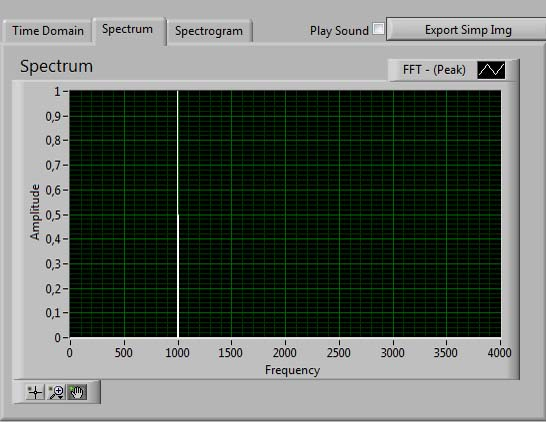
\includegraphics[height=8cm]{besselspec0}
\rule{30em}{0.5pt}
\caption[Spectrum of a 1000Hz signal]{Spectral diagram of a pure 1000Hz signal. Naturally there are no sidebands.}
\label{fig:besselspec0}
\end{figure}\\
\begin{figure}[htbp]
\centering
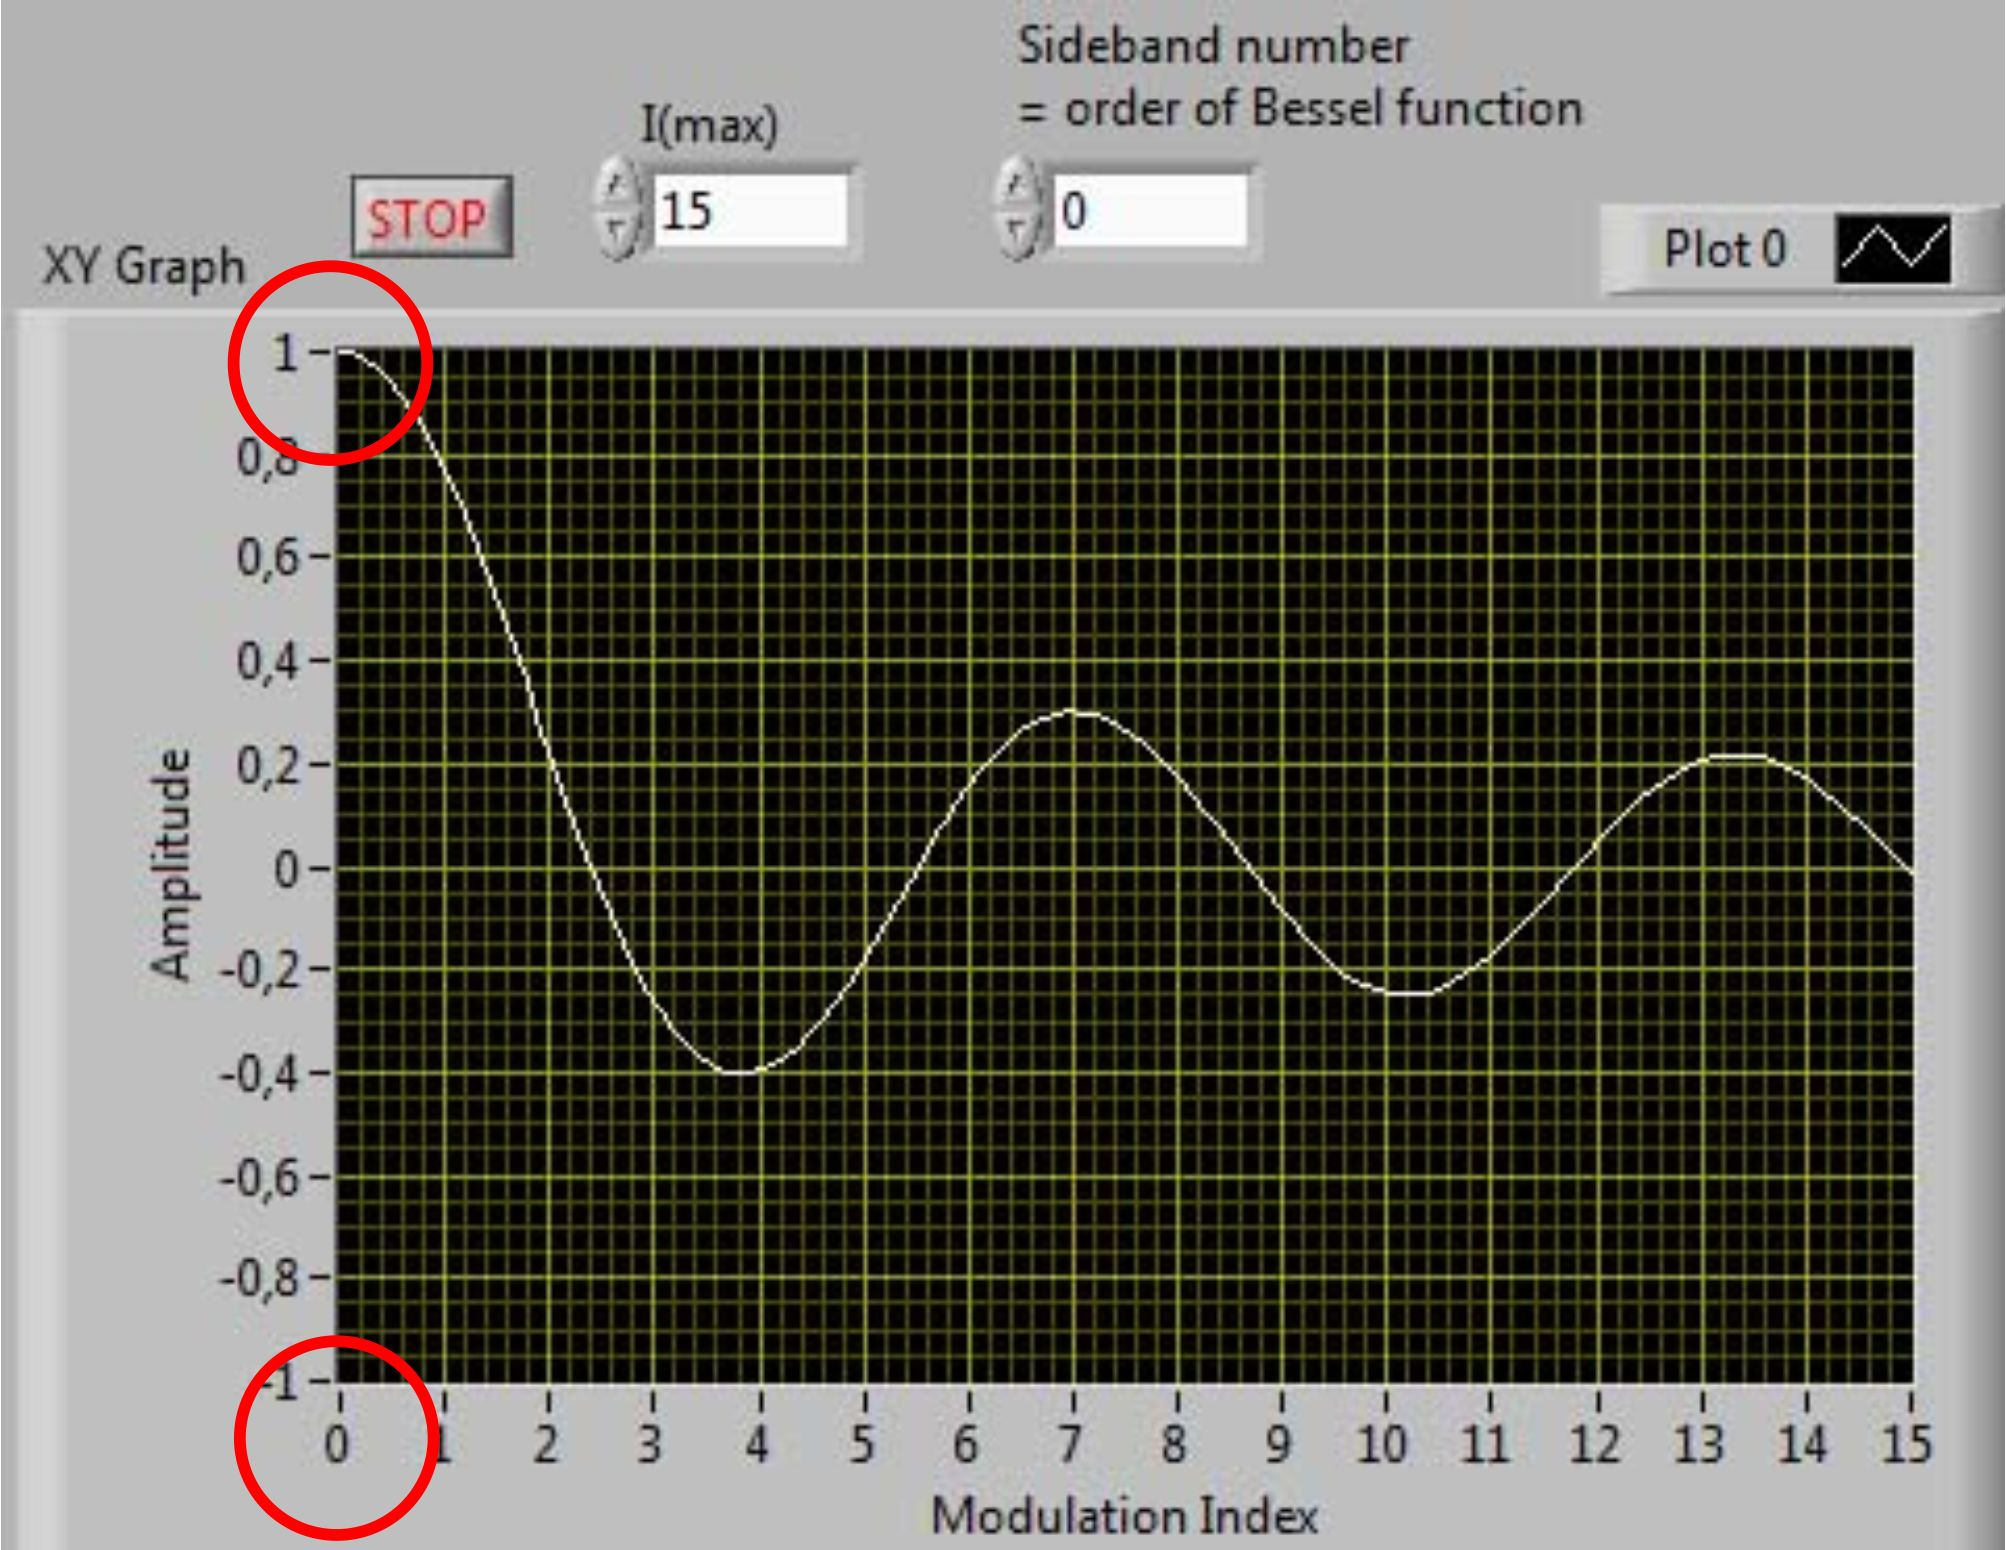
\includegraphics[height=8cm]{bessel0}
\rule{30em}{0.5pt}
\caption[Bessel function of order 0]{Bessel function of the carrier component (order 0) Remark the amplitude is equal to 1 for I = 0: $J_{0}$(0) = 1}
\label{fig:bessel0}
\end{figure}\\
\begin{figure}[htbp]
\centering
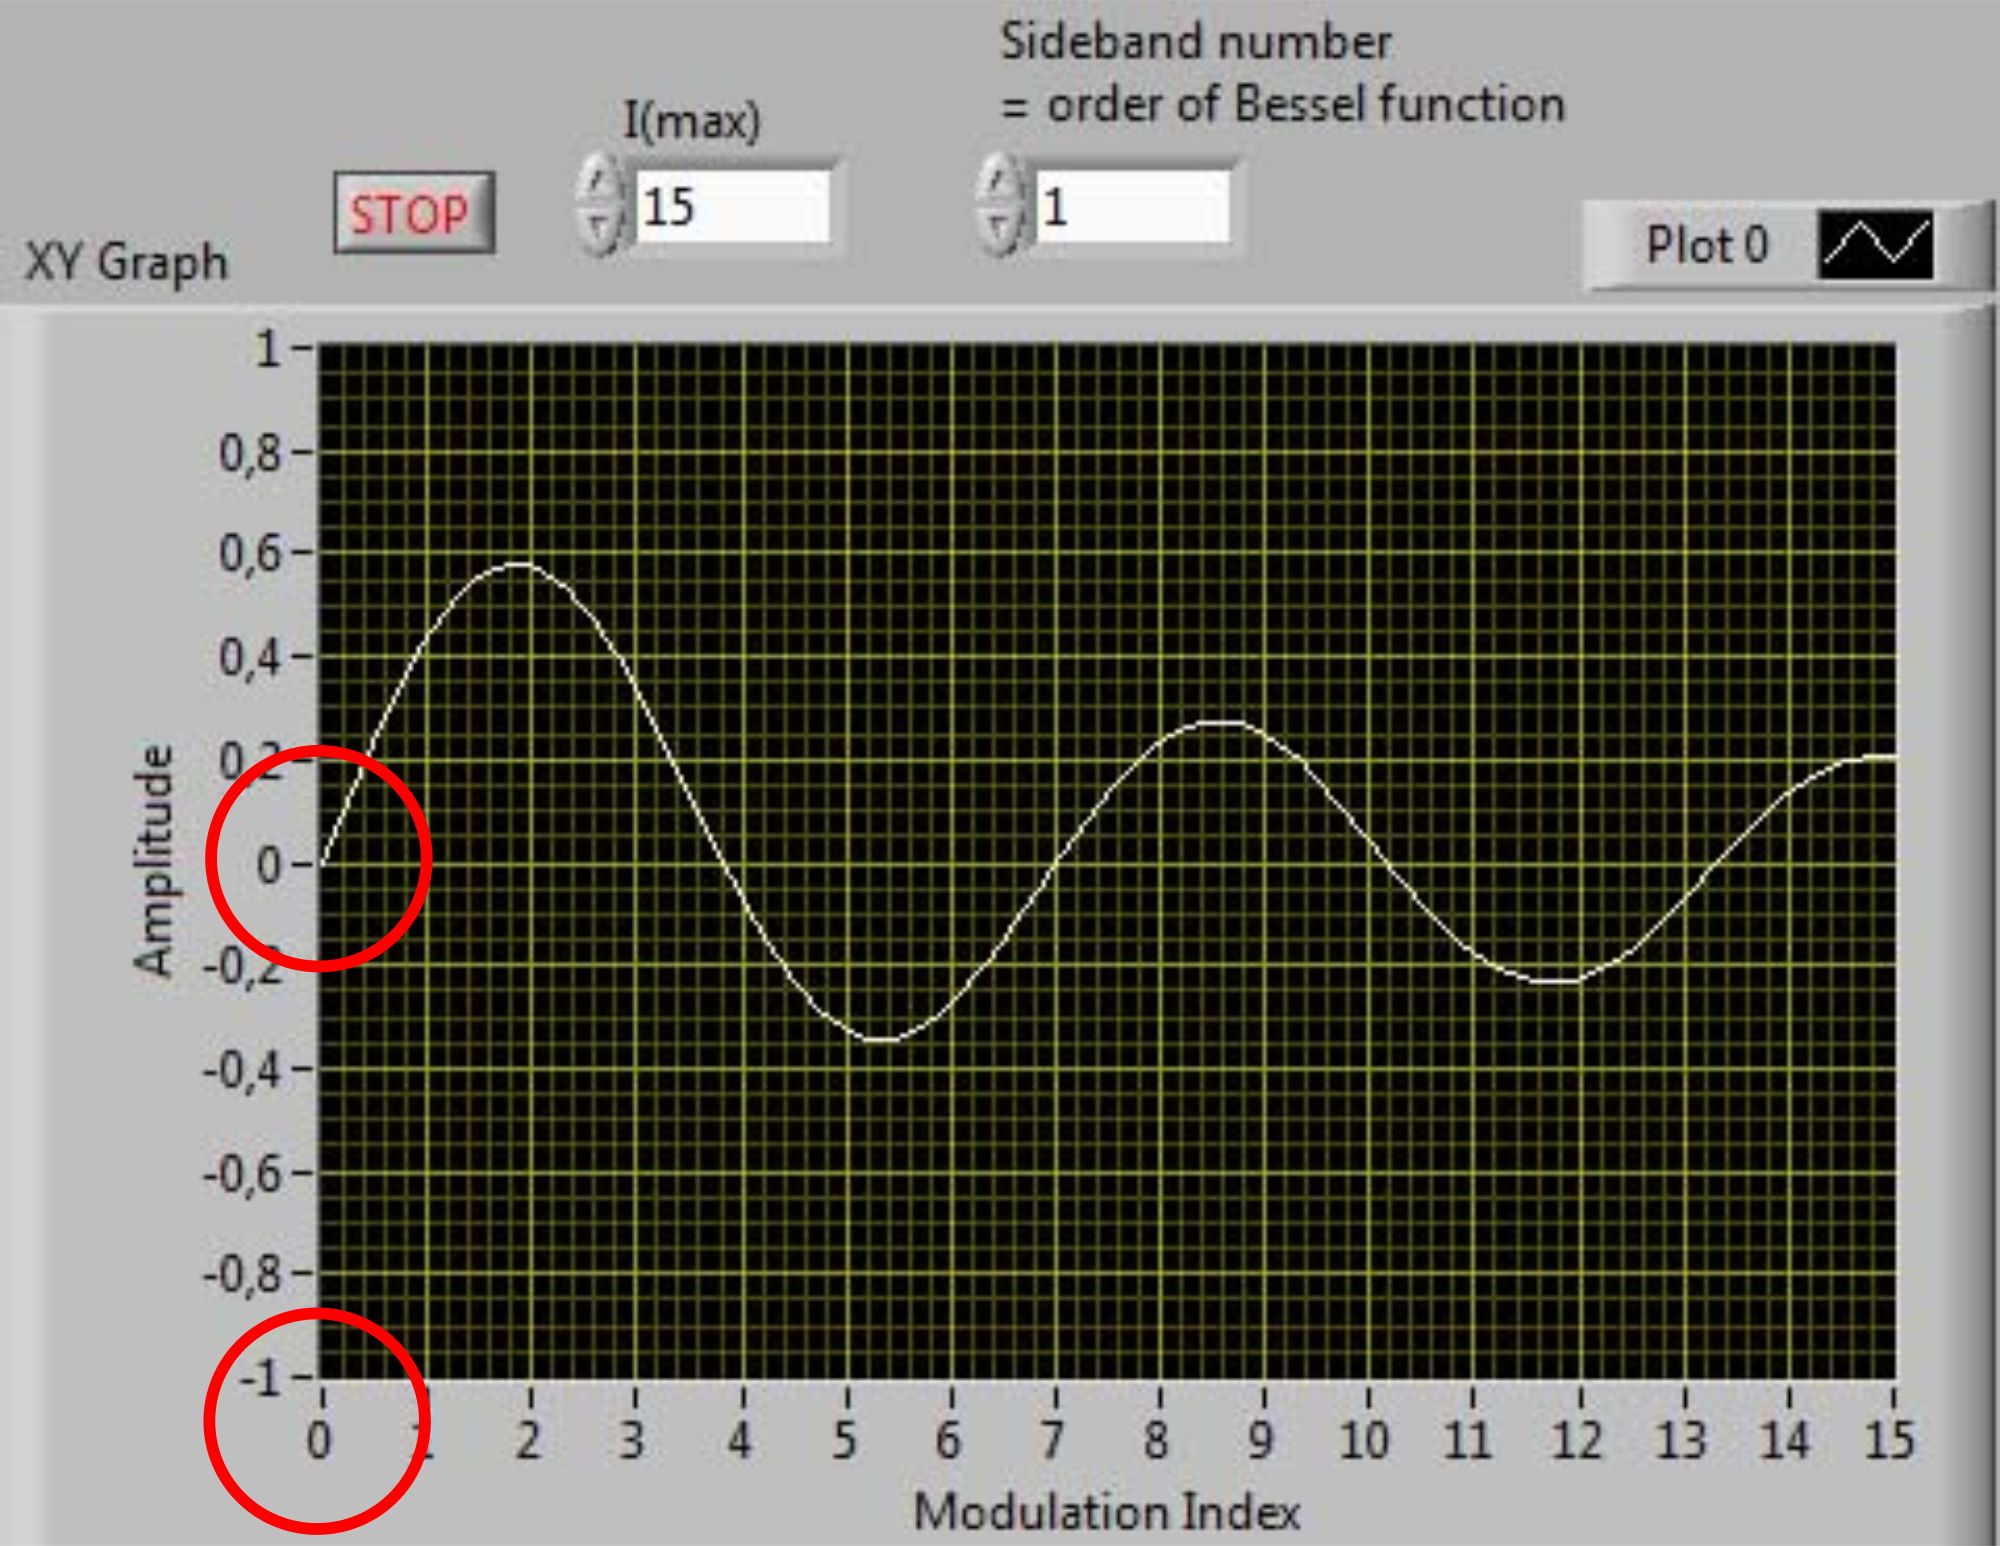
\includegraphics[height=8cm]{bessel0sideband1}
\rule{30em}{0.5pt}
\caption[Bessel function of order 1]{Bessel function of the first sidebands component (order 1) Remark the amplitude is equal to 0 for I = 0: $J_{1}$(0) = 0}
\label{fig:bessel0}
\end{figure}\\
\section{Modulation index I = 1}
\hspace{1cm} $J_{0}$(1) $<$ 1 (carrier component begins to decline) \\ 

\hspace{1cm} $J_{n}$(1) $\geq$ 0 (sidebands begin to increase)  
\begin{figure}[htbp]
\centering
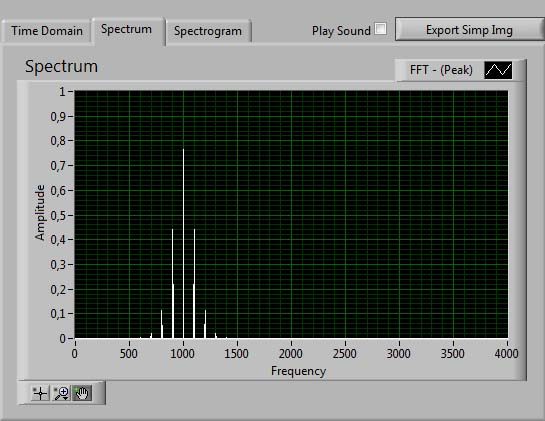
\includegraphics[height=8cm]{besselspec1}
\rule{30em}{0.5pt}
\caption[Spectrum of 1000Hz modulated with 100Hz signal]{Spectral diagram of a 1000Hz signal modulated with a 100Hz signal and I = 1.}
\label{fig:besselspec1}
\end{figure}
\begin{figure}[htbp]
\centering
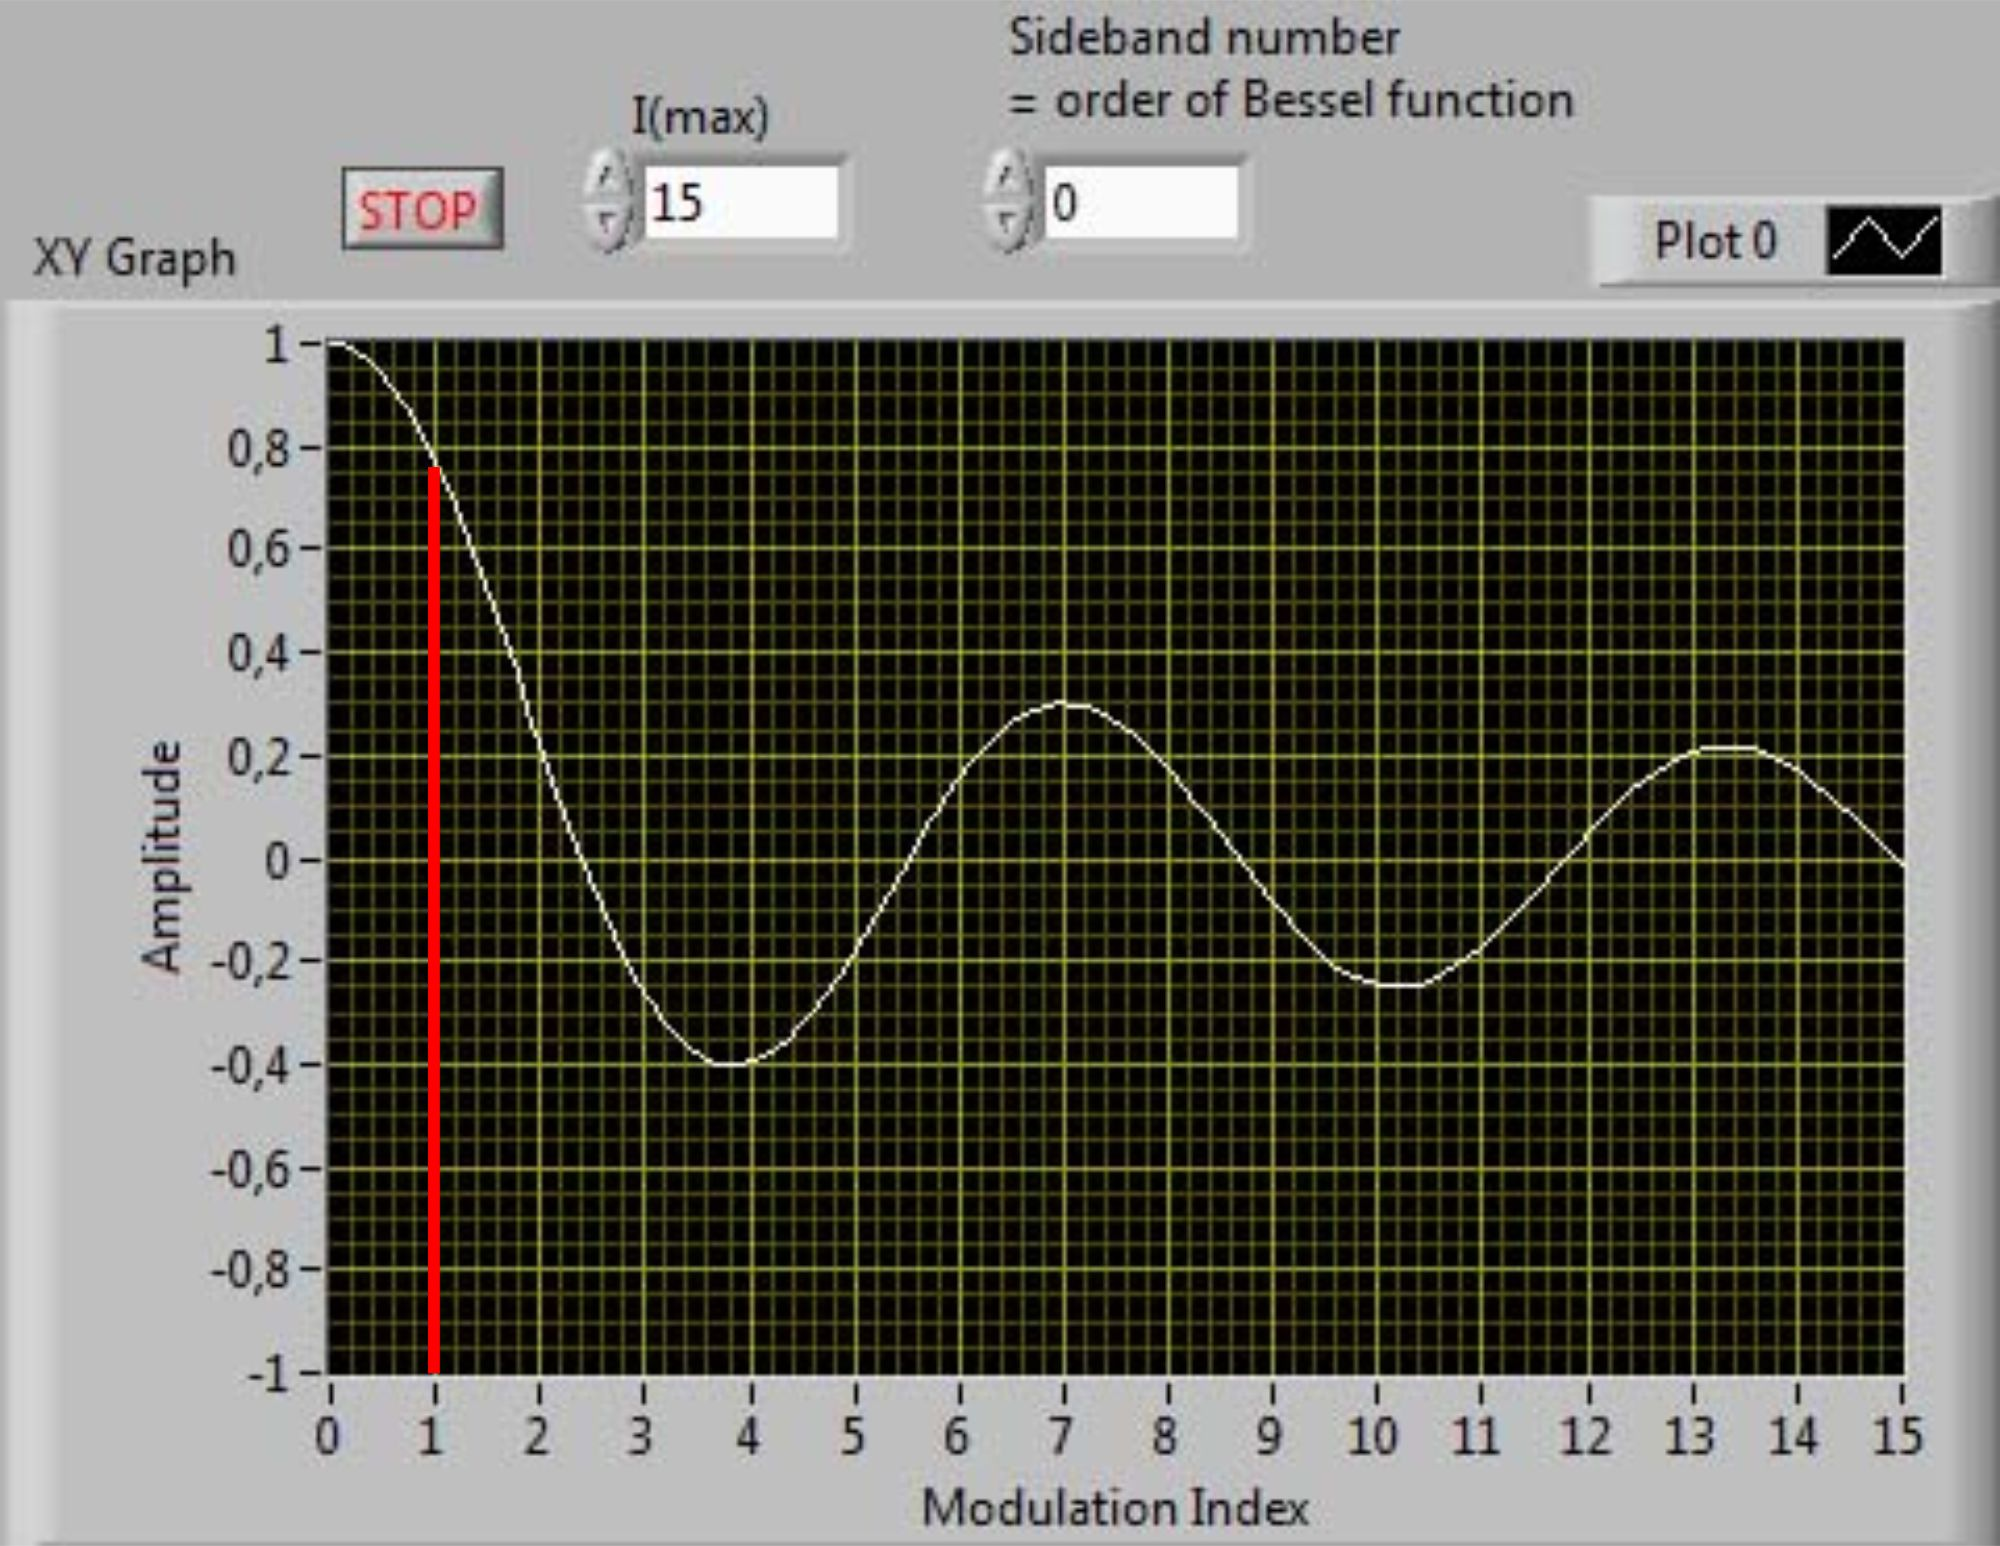
\includegraphics[height=8cm]{bessel0carrier}
\rule{30em}{0.5pt}
\caption[Bessel function of order 0, I = 1]{Bessel function for the carrier (order 0) and I = 1 shows that the amplitude of the carrier component decreases.}
\label{fig:bessel0carrier}
\end{figure}
\begin{figure}[htbp]
\centering
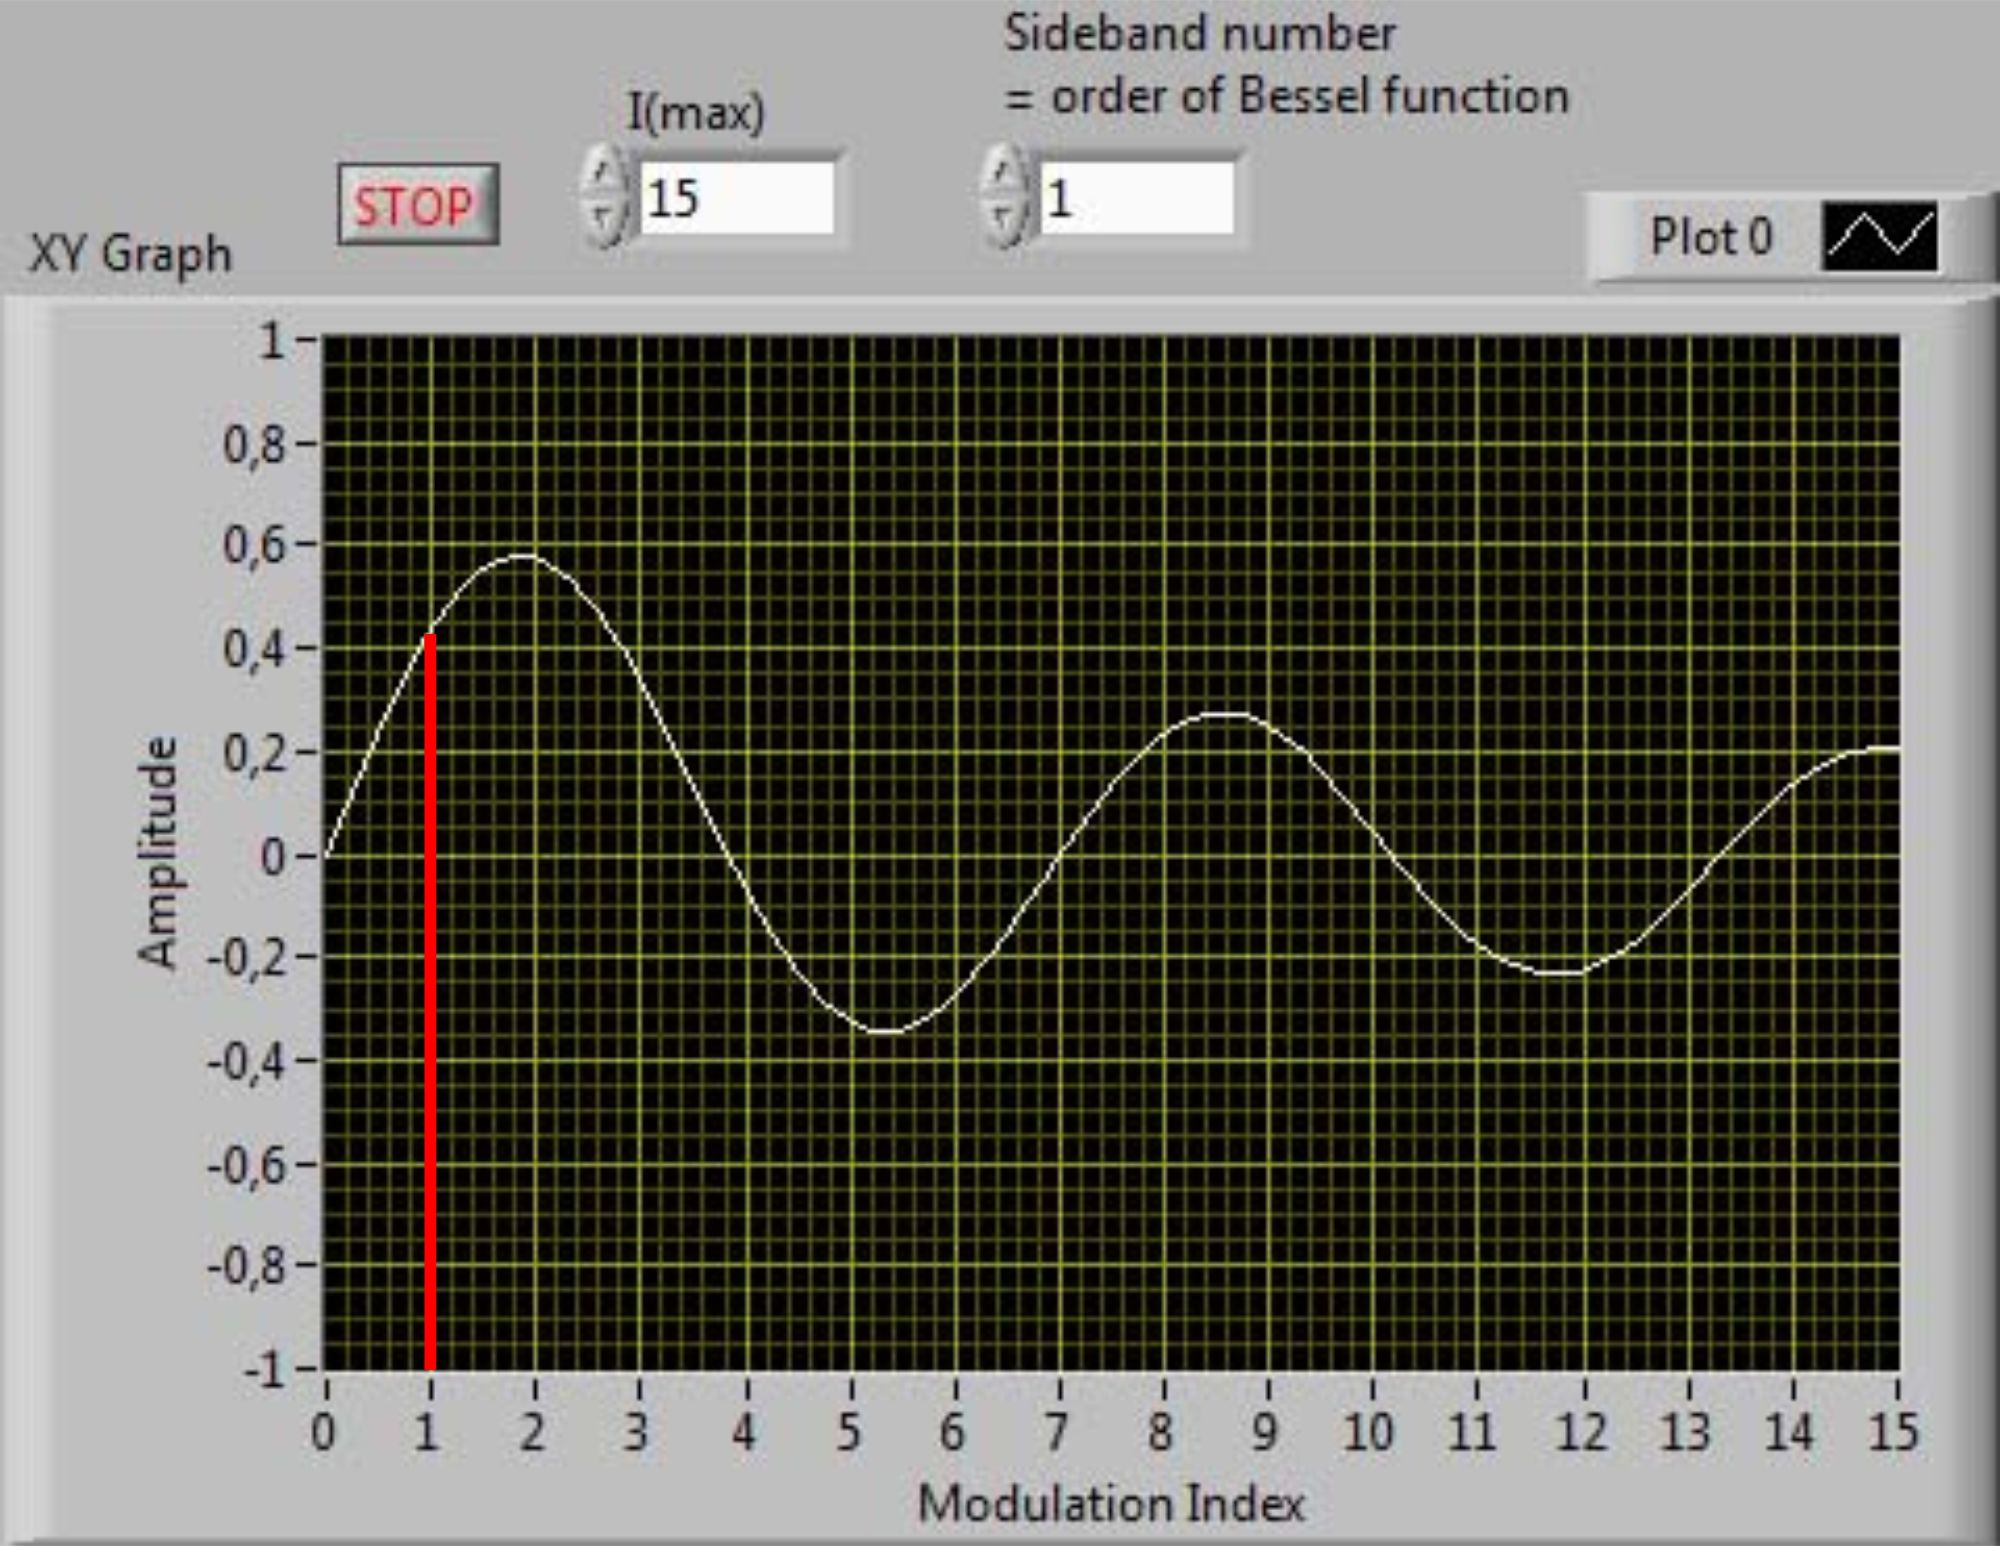
\includegraphics[height=7.5cm]{bessel11}
\rule{30em}{0.5pt}
\caption[Bessel function of order 1, I = 1]{Bessel function of the first sideband component (order 1) returns an amplitude of 0.4 if I = 1. Compare this value with figure \ref{fig:besselspec1}}
\label{fig:bessel11}
\end{figure}
\begin{figure}[htbp]
\centering
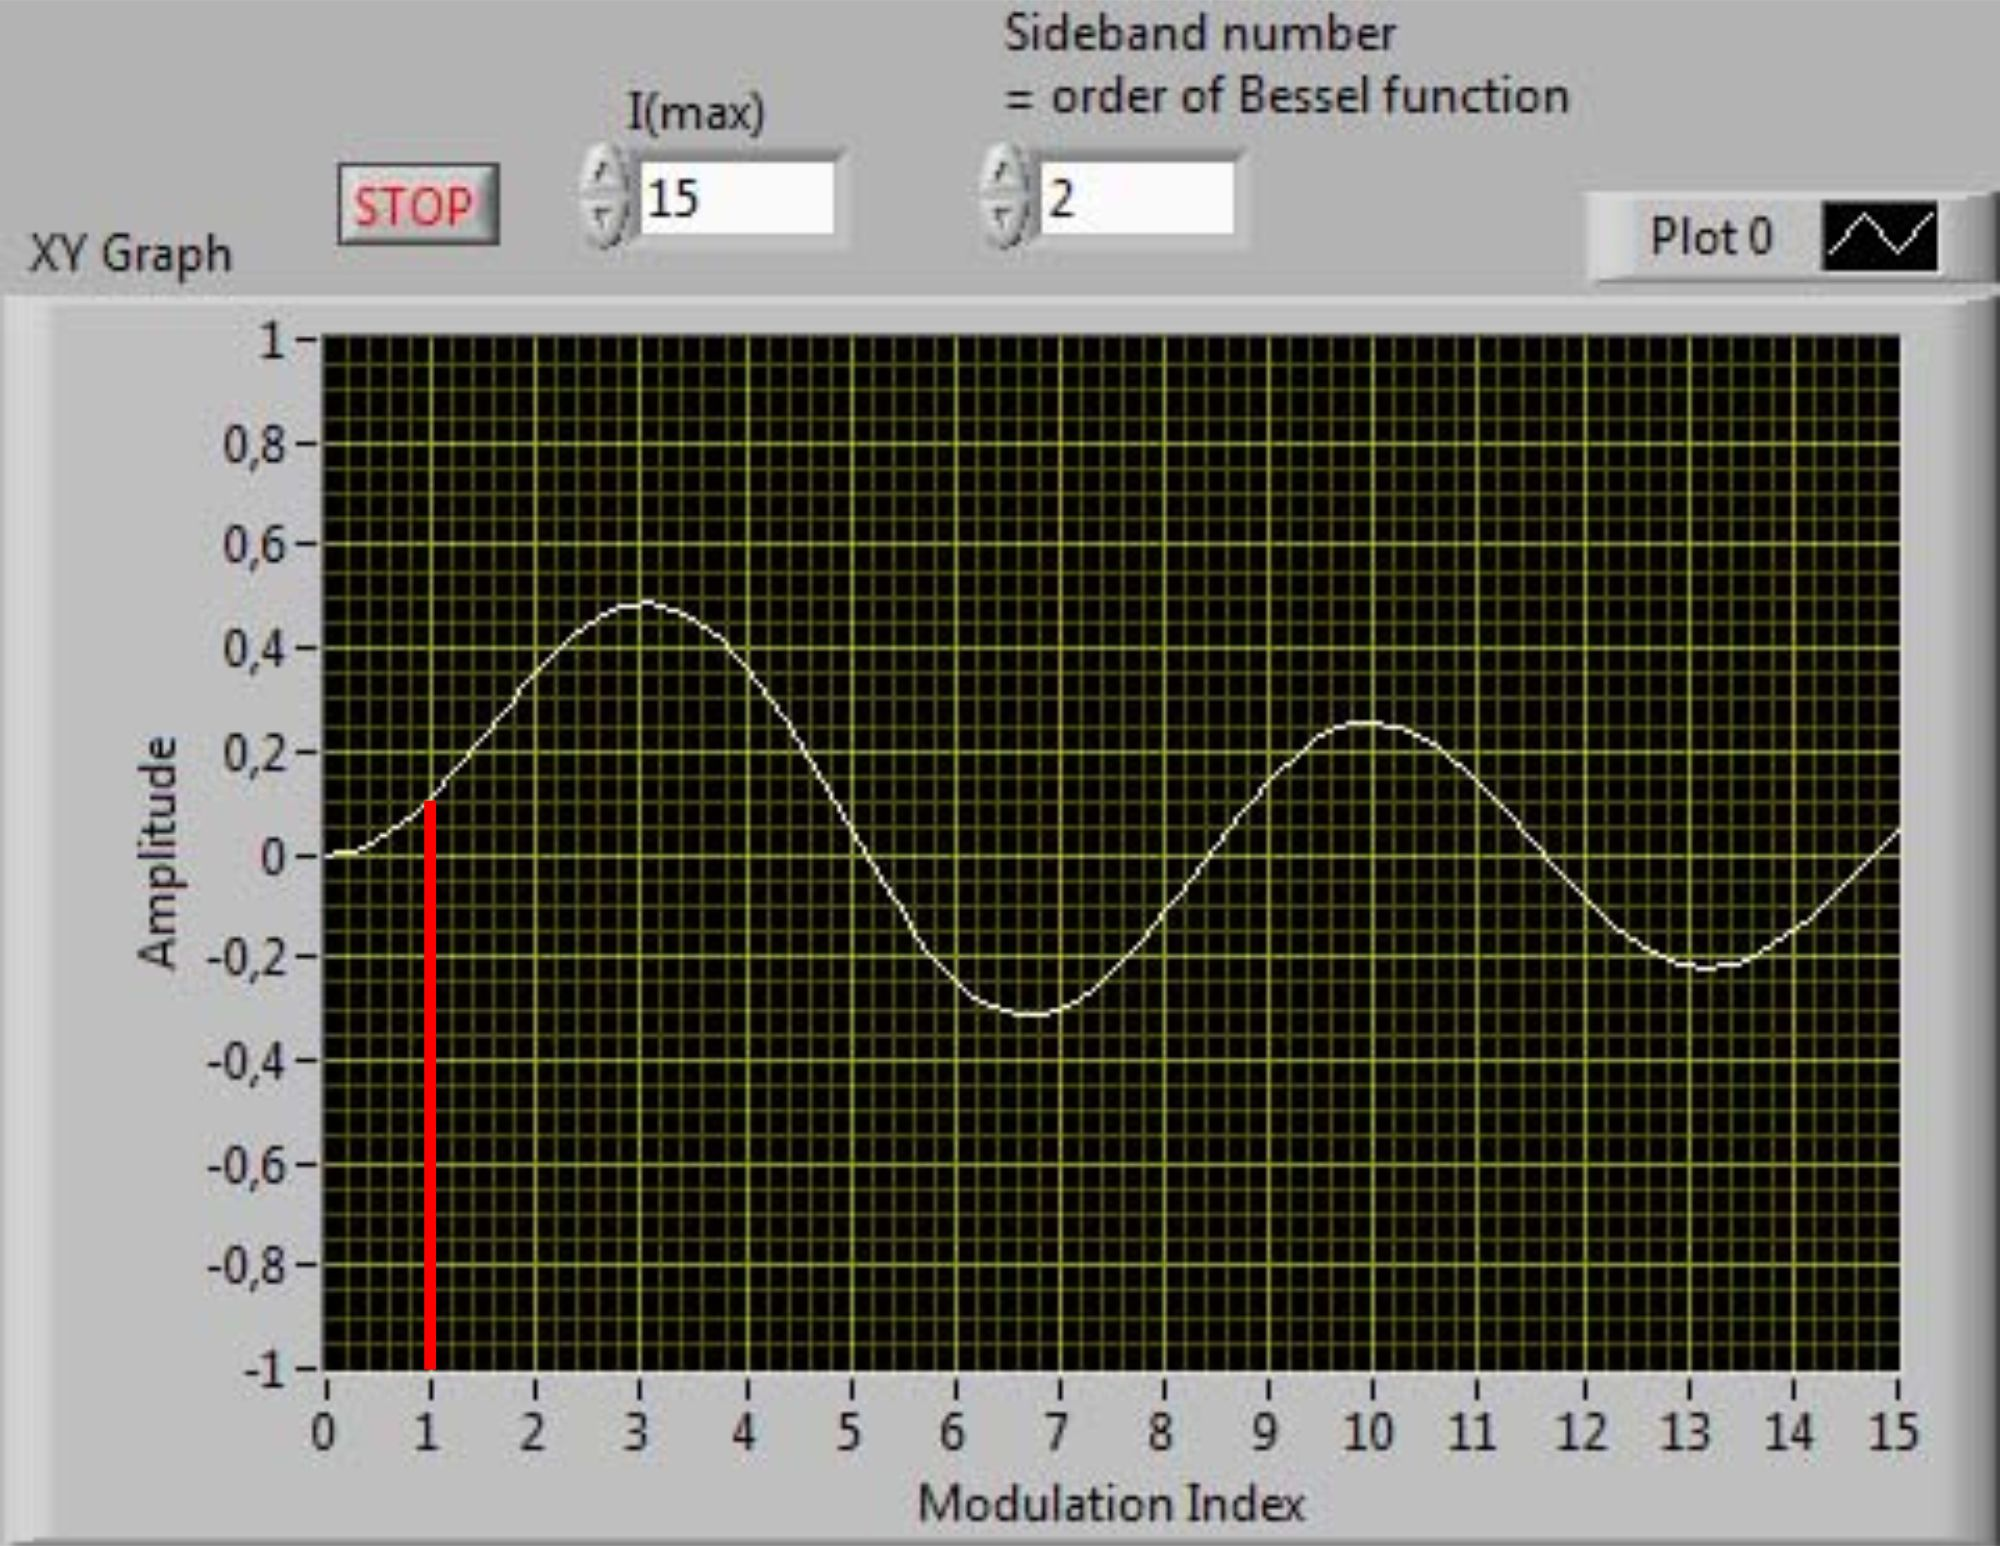
\includegraphics[height=7.5cm]{bessel21}
\rule{30em}{0.5pt}
\caption[Bessel function of order 2, I = 1]{Bessel function of the second sideband component (order 2) returns an amplitude of 0.1 if I = 1. Compare this value with figure \ref{fig:besselspec1}}
\label{fig:bessel21}
\end{figure}
\begin{figure}[htbp]
\centering
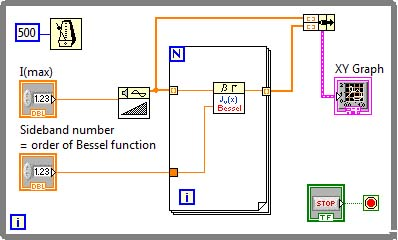
\includegraphics[height=3cm]{besselLabview}
\rule{30em}{0.5pt}
\caption[Bessel functions in Labview]{Simple labview program to display Bessel functions of the first kind}
\label{fig:besselLabview}
\end{figure}
